%% ICIIT 2027 full paper — ACM proceedings template (acmart, sigconf; the conference's .bst; Overleaf's acmart, as the
%% conference's acmart.cls v1.90a breaks with hyperxmp on TeX Live 2026).
%% Compile on Overleaf (pdfLaTeX). Numbers: shadowvale-solver, tag exp-v2 (experiments/results/exp-v2).
\documentclass[sigconf]{acmart}

\usepackage{booktabs}
\usepackage{multirow}

\settopmatter{printacmref=false}
\setcopyright{none}
\renewcommand\footnotetextcopyrightpermission[1]{}
\acmConference[ICIIT 2027]{2027 12th International Conference on Intelligent Information Technology}{March 4--7, 2027}{Ho Chi Minh City, Vietnam}

\begin{document}
\setlength{\emergencystretch}{1.5em}

\title{Do Quantum-Inspired Solvers Help Real-Time NPC Squad Coordination?\texorpdfstring{\\}{ }
A Reproducible QUBO Benchmark in a Game Testbed}

\author{Tran Tuan Anh}
\author{Nguyen Dang Khoa}
\author{Nguyen Dinh Tai}
\author{Nguyen Cong Thinh}
\author{Lai Duc Hung}
\affiliation{%
  \institution{FPT University}
  \city{Ho Chi Minh City}
  \country{Vietnam}}
\email{anhttse184743@fpt.edu.vn}

\renewcommand{\shortauthors}{Tran et al.}

\begin{abstract}
When a squad of game guards spots the player, each guard must pick a position, and the choices
interact. We formulate this assignment as a QUBO in our stealth game ShadowVale and ask whether
quantum and quantum-inspired solvers help within the 120\,ms a re-plan may take. On 3{,}447 QUBOs
recorded in play, 1{,}350 generated instances of up to 1{,}200 variables, Moving AI maps and QAPLIB,
we compare ten solvers against exact references. Only travel cost depends on the agent, so the exact problem reduces to
choosing a node set plus a Hungarian assignment, which proves every game-size optimum in about
0.1\,s. Classical tabu search is optimal in 99.9\,\% of game runs, and one millisecond of local
search after Greedy cuts its gap from 2.8\,\% to 0.27\,\%. The quantum-inspired QIEA is no more
accurate than a genetic algorithm or than PBIL, its Q-bit-free ablation; bit-flip annealers (SA,
SQA) trail Greedy; and simulated QAOA, read from the statevector, does not find the optimum more
often than uniform sampling of valid assignments. In 2{,}100 paired replays of scripted exploits on the final build, the solver changed
capture rates by up to 36 points against one exploit, but in opposite directions across exploits.
\end{abstract}

\ccsdesc[500]{Computing methodologies~Multi-agent planning}
\ccsdesc[500]{Theory of computation~Discrete optimization}
\ccsdesc[300]{Applied computing~Computer games}
\ccsdesc[100]{Hardware~Quantum computation}

\keywords{QUBO, NPC coordination, game AI, quantum-inspired optimization, QAOA, tabu search, benchmark}

\maketitle

\section{Introduction}

When a squad of non-player characters (NPCs) spots the player, each guard must pick a position: one
that covers an escape route, is not redundant with its comrades' positions, flanks the player where
possible, and is not too far away. These choices interact, so they form a combinatorial
assignment problem rather than a set of independent decisions. Commercial games usually score
positions per agent and assign them greedily~\cite{Straatman2005,Orkin2006,Jack2013}. The
interactions are pairwise, which makes the problem a quadratic assignment problem (QAP), NP-hard in
general~\cite{Sahni1976}, and a natural candidate for Quadratic Unconstrained Binary Optimization
(QUBO)~\cite{Lucas2014,Glover2019}, the input format of quantum annealers, of the Quantum Approximate
Optimization Algorithm (QAOA)~\cite{Farhi2014}, and of many quantum-inspired heuristics.

This paper asks whether that route pays off at the scale and latency of a real game. We
formulate squad position assignment in our stealth game ShadowVale as a QUBO, solve it under the
120\,ms the game allows for a re-plan with ten classical, quantum-inspired and simulated-quantum
solvers, score them against exact optima on recorded, generated and public instances, and measure
with scripted exploit bots whether the choice of solver changes play.

The answer is mostly negative for the quantum side, and we report it as such. Our contributions are:
(1)~a QUBO for tactical position assignment with a penalty weight that provably keeps every
optimum feasible; (2)~the observation that only travel cost depends on the agent, which reduces the
exact problem to choosing a node set plus a Hungarian assignment and yields proven optima for every
game-size instance; (3)~a reproducible benchmark (code, instances, tuning and raw results are
public~\cite{ShadowValeSolver}) showing that, at game scale, a cheap classical local search is
enough, that QIEA is no more accurate than a genetic algorithm or than its Q-bit-free ablation, and
that QAOA does not beat uniform sampling of valid assignments; and (4)~a paired gameplay evaluation
showing that the solver can change capture rates against a given exploit, but not consistently, so
that better optimization of the objective is not a reliable proxy for a stronger opponent.

\section{Related Work}

Games choose combat positions per agent by scoring waypoints or queries~\cite{Straatman2005,Jack2013}
on top of FSM or planning agents~\cite{Orkin2006,Yannakakis2018}, ignoring pairwise effects or
handling them greedily. Assigning agents to positions with interacting values relates to
weapon--target assignment~\cite{Ahuja2007}, multi-robot task allocation~\cite{Gerkey2004} and the
QAP, for which robust tabu search is a strong baseline~\cite{Taillard1991,Loiola2007}. One-hot
penalties turn assignment problems into QUBOs~\cite{Lucas2014,Glover2019}; quantum annealing has
been applied to similar route-choice problems~\cite{Neukart2017}, while quantum work in games has
focused on content generation~\cite{Wootton2020}. QAOA's transverse-field mixer explores all $2^n$
bit strings, whereas constraint-preserving mixers stay in the one-hot sector~\cite{Hadfield2019,Wang2020XY};
SQA simulates a transverse-field annealer by path-integral Monte Carlo~\cite{Martonak2002,Kadowaki1998};
QIEA samples bits from rotating Q-bits~\cite{HanKim2002}, much like PBIL~\cite{Baluja1994}. We know of
no study comparing these families with strong classical baselines on NPC coordination under a game
latency budget.

\section{Problem and QUBO Formulation}

A re-plan concerns a combat group of $A$ agents (2--8 in play) and a local subgraph $V$ of the
tactical navigation graph of at most 24 nodes: every agent's current node, filled up with the
nodes nearest to the player's last known position (in play $19 \le |V| \le 24$, so $n=A|V|\le192$). A plan is an injective map
$\sigma$ from agents to nodes (one node per agent, no node shared). With escape nodes $X \subseteq V$
(the subgraph's boundary and map chokepoints) and line of sight ray-cast once per map load, the
objective is
\begin{multline}\label{eq:F}
F(\sigma) = \sum_a \big(w_c\,\mathrm{cov}_{\sigma_a} + w_q\, q_{\sigma_a} - w_d\, d_{a,\sigma_a}\big)\\
 + \sum_{a<b} \big(w_f\,\mathrm{flk}_{\sigma_a\sigma_b} - w_r\,\mathrm{ovl}_{\sigma_a\sigma_b}\big),
\end{multline}
where $\mathrm{cov}_r$ counts escape nodes visible from $r$, $q_r \in [0,1]$ is the cover quality of
$r$ facing the player, $d_{a,r}$ is agent $a$'s travel cost in hops, $\mathrm{ovl}_{rr'}$ counts escape
nodes visible from both $r$ and $r'$, and $\mathrm{flk}_{rr'}=1$ when $r$ and $r'$ lie on opposite
sides of the player. The weights $(w_c,w_r,w_f,w_q,w_d)=(1,0.5,1,0.5,0.1)$ come from the game's
content bundle; they were set by hand, and we did not analyse their sensitivity.

With $x_{a,r}=1$ iff $\sigma_a=r$ ($n=A|V|$ binary variables) the QUBO energy is
\begin{equation}\label{eq:E}
E(x) = -F(x) + \lambda\sum_a\Big(\sum_r x_{a,r}-1\Big)^2 + \lambda\sum_r\sum_{a<b}x_{a,r}x_{b,r},
\end{equation}
so $E=-F$ on every feasible $x$, and gaps below are computed on $F$.

\textbf{Penalty weight.} With $L=\max_r(w_c\mathrm{cov}_r+w_q q_r)$, $D=w_d\max d$,
$P^+=w_f\max\mathrm{flk}$, $P^-=w_r\max\mathrm{ovl}$ we set
$\lambda = 1 + L + 2(A-1)P^+ + D + (A-1)P^-$. Any infeasible $x$ is repaired by steps that each lower
$E$: (i)~an agent with $k\ge2$ nodes drops one (penalty $-\lambda$ or more, reward at most
$L+2(A-1)P^+$); (ii)~of two agents sharing a node, one moves to a free node (penalty $-\lambda$, $F$
changes by at most $L+D+(A-1)(P^+ + P^-)$); (iii)~an agent without a node takes a free one (loss at
most $D+(A-1)P^-$). So every global minimum is feasible; single-flip local minima need not be, as
(ii) is a two-bit move. Tests check the dominance exhaustively on small instances.

\textbf{Node-only structure.} In Eq.~\eqref{eq:F} only $d_{a,r}$ depends on the agent. Writing
$S=\sigma(\{1..A\})$,
\begin{equation}\label{eq:set}
\max_\sigma F = \max_{|S|=A}\Big[G(S) - w_d \min_{\pi: \text{agents}\leftrightarrow S}\sum_a d_{a,\pi(a)}\Big],
\end{equation}
with $G(S)$ the node-only terms. The inner problem is a linear assignment, solved exactly by the
Hungarian method~\cite{Kuhn1955}. There are $\binom{|V|}{A}=134{,}596$ node sets for $A=6$,
$|V|=24$, against $|V|!/(|V|-A)! \approx 9.7\times10^7$ assignments. Our exact solver
\texttt{exact\_set} reads this structure from $Q$ alone (it checks that all agent pairs share one
symmetric block), ranks sets by $G(S)$ plus a lower bound on the assignment cost, and solves
assignments in that order until the bound passes the incumbent; it proves the optimum of a 6-agent,
24-node instance in about 0.1\,s, against 1--5\,s for our earlier branch and bound. The structure
also bears on QAOA: the one-hot encoding needs $A|V|$ qubits although the hard part of the problem
is the choice of $S$ over $|V|$ nodes (Section~\ref{sec:disc}).

\section{Solvers and Experimental Setup}\label{sec:setup}

Every solver receives only the QUBO matrix and the layout $(A,|V|)$ and returns a bit vector; the
energy is computed on $Q$ for all of them. Stochastic solvers stop at 80\,\% of the budget, so that
the reply reaches the game in time.

\textbf{Classical.} \emph{Greedy} places agents in index order on the free node of lowest marginal
energy; the game runs it in-process as fallback. Three new solvers move only between assignments,
by moving one agent to a free node or swapping two, each evaluated in $O(1)$: \emph{Greedy+LS}
(steepest descent from Greedy), \emph{Tabu} (random tenure and aspiration as in robust tabu
search~\cite{Taillard1991,Glover1989}, restarts with a perturbation), and \emph{SA-1h} (Metropolis
annealing). \emph{GA} evolves assignments (tournament, uniform crossover with repair, mutation,
elitism); \emph{SA} is dwave-neal~\cite{DWaveNeal,Kirkpatrick1983} on raw bits.
\textbf{Quantum-inspired and simulated quantum.} \emph{QIEA}~\cite{HanKim2002} samples bits from
rotating Q-bits; \emph{PBIL} (new) is QIEA with the rotation replaced by a PBIL probability
vector~\cite{Baluja1994}, isolating the Q-bit. \emph{SQA} is path-integral Monte Carlo with 16
Trotter replicas~\cite{Martonak2002}; \emph{QAOA}~\cite{Farhi2014} as a solver ($p=2$, 512 shots) is an exact
numpy statevector simulation up to 18 qubits; a separate study (Section~\ref{sec:qaoa}) reads
$p=1$--3 circuits directly from the statevector, with angles from a grid plus Nelder--Mead and no
time limit, for the standard and a ring-XY mixer. GA, QIEA, PBIL, Tabu and SA-1h start from Greedy's
assignment; SA, SQA and QAOA from random states.
\textbf{Exact references.} Enumeration, \texttt{exact\_set} (Eq.~\ref{eq:set}) up to
$5\times10^6$ node sets, otherwise branch and bound.

\textbf{Repair and feasibility.} An output is \emph{raw feasible} if it is an injective assignment
before repair. Infeasible bits from SA, SQA and QAOA are repaired (per agent, the on-bit of lowest
marginal energy, then the cheapest free node), at about Greedy's cost, outside the reported latency.

\textbf{Instances.} (i)~\emph{Game}: 4{,}549 QUBOs recorded during scripted play on Map~1 (2--8 agents,
19--24 nodes, 44--184 variables); a hashed quarter (1{,}102) is the tuning split and the other
3{,}447 are evaluated. (ii)~\emph{Full}: generated instances with $|V|\in\{20,\dots,100\}$,
$A\in\{4,8,12\}$, chokepoint density $\{0,0.3,0.6\}$, 30 seeds per cell (1{,}350 instances, up to
1{,}200 variables). (iii)~\emph{Small}: $|V|\in\{6,8,10\}$, $A\in\{2,3\}$ (180 instances, 12--30
variables), where QAOA can run. (iv)~\emph{Moving AI}: 342 coordination instances built on
game maps~\cite{Sturtevant2012}. (v)~\emph{QAPLIB}: the 77 instances with $n\le30$
facilities~\cite{Burkard1997}, scored against the published optimum (76; one has optimum 0).

\textbf{Protocol.} All solvers get the same 120\,ms wall-clock budget on one CPU thread (Intel
i5-13450HX, 16\,GB, Python 3.11, numpy 2.4, dwave-neal 0.6); QAPLIB is also run at 1\,s. Repeats:
3 per game, full and Moving AI instance, 5 per small and QAPLIB instance, with independent seeds.
GA, SA, SQA, QIEA, PBIL, Tabu and SA-1h were each tuned with the same effort (30 random
configurations including the default, the best three re-run three times) on the tuning split and
on generated seeds 901+, which the evaluation excludes. The optimality gap is
$(F^\star-F)/|F^\star|$, where $F^\star$ is the proven optimum (all game, small and Moving AI
instances, and the full-suite instances with at most $5\times10^6$ node sets) or, otherwise,
the best of two independent 2\,s runs (Tabu and GA); a solver run that beats this reference gets a
negative gap. For each pair of solvers we average the repeats of an instance first and apply the
Wilcoxon signed-rank test over instances, Holm-corrected~\cite{Holm1979}; we report differences in
percentage points (pp) with bootstrap 95\,\% intervals, and treat differences below 0.1\,pp as
practically negligible however small $p$ is. Benchmark parts ran as concurrent single-threaded processes; latency figures are
checked against an idle-machine re-run (Section~\ref{sec:disc}).

\textbf{Gameplay replay.} A scripted bot attacks one camp of Map~1 with one of three exploits:
\emph{same\_route} crosses on a fixed lane and flees after a reaction time, \emph{same\_bush} hides in
the same bush, \emph{stone\_lure} throws a stone to one side and sneaks past on the other. Each
bot's time knob was calibrated on Greedy (seeds 500+) to about 50\,\% capture on the final build
before any comparison. Every variant plays the same 100 seeds per bot (1000+) at a fixed 30\,fps
step, applying each plan after its real solve latency (lockstep); \emph{none} keeps radio alerts
but no plans. Captures are compared on paired seeds with the exact McNemar test, escape time and
coverage (share of escape nodes seen from the plan) with Wilcoxon, all Holm-corrected against
Greedy and against \emph{none}.

\section{Results}\label{sec:results}

\begin{table*}[t]
\centering\small
\caption{All solvers at the 120\,ms budget. Gap: mean optimality gap per instance (repeats averaged
first). Opt.: share of runs at the proven optimum. p50: median latency. Evals: median number of
candidate evaluations per run (moves for Greedy+LS, Tabu and SA-1h; samples otherwise). Raw feas.:
share of the solver's own samples that were valid assignments before repair. Full: generated
instances up to 1{,}200 variables, gap to the proven optimum or to an independent 2\,s reference.
QAPLIB: gap to the published optimum.}
\label{tab:solvers}
\begin{tabular}{lrrrrrrrrr}
\toprule
 & \multicolumn{5}{c}{Recorded game instances} & Full & Moving & \multicolumn{2}{c}{QAPLIB} \\
\cmidrule(lr){2-6}\cmidrule(lr){7-7}\cmidrule(lr){8-8}\cmidrule(lr){9-10}
Solver & gap & opt. & p50 & evals & raw & gap & AI gap & 120\,ms & 1\,s \\
 & \% & \% & ms & & feas.\,\% & \% & \% & \% & \% \\
\midrule
Greedy & 2.76 & 39.5 & 0.13 & -- & 100 & 8.18 & 10.20 & 73.1 & 73.1 \\
Greedy+LS & 0.27 & 74.7 & 0.40 & 144 & 100 & 1.32 & 0.50 & 15.3 & 10.4 \\
Tabu & 0.000 & 99.9 & 96.1 & 77{,}550 & 100 & 0.78 & 0.00 & 7.5 & 1.5 \\
GA & 0.11 & 78.2 & 96.1 & 1{,}966 & 100 & 2.70 & 0.56 & 19.7 & 9.5 \\
SA (bits) & 3.91 & 34.7 & 98.9 & 136 & 100 & 29.52 & 9.06 & 66.1 & 46.6 \\
SA-1h & 0.087 & 80.3 & 95.9 & 2{,}854 & 100 & 2.75 & 0.50 & 16.1 & 5.2 \\
PBIL & 0.036 & 90.4 & 96.1 & 1{,}474 & 15 & 2.14 & 0.86 & 28.5 & 13.1 \\
SQA & 4.10 & 33.0 & 84.0 & 640 & 63 & 32.30 & 9.76 & 92.2 & 63.9 \\
QIEA & 0.11 & 82.1 & 96.1 & 1{,}028 & 0 & 2.19 & 2.57 & 26.4 & 14.8 \\
\bottomrule
\end{tabular}

\end{table*}

\subsection{Solution quality on game and generated instances}

On the 3{,}447 recorded game instances, all with a proven optimum (Table~\ref{tab:solvers}), tabu
search is optimal in 99.9\,\% of the runs. Greedy is 2.76\,\% from the optimum on average; one
millisecond of local search (Greedy+LS, median 0.40\,ms) cuts this to 0.27\,\%. PBIL, SA-1h, GA and
QIEA lie between 0.04 and 0.11\,\%; QIEA and GA are indistinguishable (difference $+0.001$\,pp, 95\,\%
CI $[-0.009, 0.010]$, $p=0.42$), and PBIL's lead over QIEA (0.07\,pp, $p_\text{Holm}<10^{-70}$) is
statistically clear but practically negligible. Bit-flip SA and SQA are worse than Greedy (3.9 and
4.1\,\%) in the same time; 63\,\% of SQA's samples are valid assignments, and QIEA's and PBIL's raw
bit samples almost never are (0 and 15\,\%).

\begin{figure}[t]
\centering
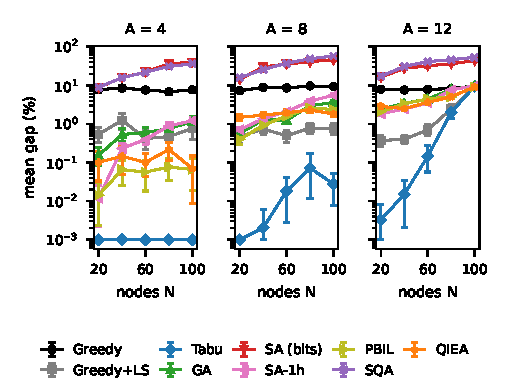
\includegraphics[width=\linewidth]{figures/full_quality.pdf}
\Description{Three panels, for 4, 8 and 12 agents, plot each solver's mean optimality gap on a log scale against the number of nodes; tabu search is lowest, bit-flip SA and SQA highest.}
\caption{Full suite: mean gap per instance by number of nodes, one panel per number of agents
(log scale; error bars: bootstrap 95\,\% CI; a gap of 0 is drawn at $10^{-3}$\,\%).}
\label{fig:full}
\end{figure}

On the full suite (Fig.~\ref{fig:full}; reference proven for 630 instances, an independent 2\,s
run for 720, never beaten at 120\,ms), tabu search is again best (0.78\,\%, at the reference in
88\,\% of runs), then Greedy+LS (1.32\,\%), PBIL (2.14\,\%), QIEA (2.19\,\%, $p=0.27$ against PBIL),
GA (2.70\,\%) and SA-1h (2.75\,\%); Greedy stays near 8\,\%. With 4 agents tabu search is exact up to
100 nodes; with 12 agents and 100 nodes every method ends near Greedy (9.0--9.6\,\%), as our Python
iterations no longer fit many times into 120\,ms. SA and SQA degrade to 36--57\,\%, and on an idle
machine bit-flip SA exceeds the budget in 34\,\% of its runs (dwave-neal's batches cannot be
interrupted).

\subsection{Public datasets}

On Moving AI coordination instances (342, proven optima) the ranking of the game
instances holds: tabu search 0.002\,\%, SA-1h and Greedy+LS 0.50\,\%, GA 0.56\,\%, PBIL 0.86\,\%,
QIEA 2.57\,\%, and the bit-flip samplers about 9\,\%, close to Greedy (10.2\,\%). QAPLIB is much harder:
at 120\,ms tabu search is 7.5\,\% from the published optimum, against 19.7\,\% for GA and 26.4\,\% for
QIEA, and with 1\,s it reaches 1.5\,\% (GA 9.5\,\%, QIEA 14.8\,\%). GA is thus far from the strongest classical
baseline, and our tabu search is in the range expected of robust tabu search on these
sizes~\cite{Taillard1991}.

\subsection{QAOA against uniform sampling}\label{sec:qaoa}

\begin{table}[t]
\centering\small
\caption{QAOA read from the statevector ($p=3$, angles optimized without a time limit),
means over instances. $P_\text{valid}$, $P_\text{opt}$: probability of measuring a valid assignment,
an optimal one. Ratio: median of $P_\text{opt}$ over that of sampling valid assignments uniformly.
hit$_{512}$, unif.: probability that 512 shots contain the optimum, for QAOA and for 512 uniformly
drawn valid assignments. X: standard mixer; XY: ring-XY mixer in the one-hot sector.}
\label{tab:qaoa}
\setlength{\tabcolsep}{3pt}
\begin{tabular}{rrlrrrrr}
\toprule
$n$ & $A{\times}|V|$ & mixer & $P_\text{valid}$ & $P_\text{opt}$ & ratio & hit$_{512}$ & unif. \\
\midrule
12 & 2$\times$6 & X & 0.35 & 0.0144 & 0.39 & 1.00 & 1.00 \\
12 & 2$\times$6 & XY & 1.00 & 0.0519 & 1.13 & 1.00 & 1.00 \\
16 & 2$\times$8 & X & 0.34 & 0.0075 & 0.35 & 0.97 & 1.00 \\
16 & 2$\times$8 & XY & 0.97 & 0.0243 & 0.97 & 0.99 & 1.00 \\
18 & 3$\times$6 & X & 0.17 & 0.0018 & 0.19 & 0.59 & 0.99 \\
18 & 3$\times$6 & XY & 0.95 & 0.0103 & 1.14 & 0.98 & 0.99 \\
20 & 2$\times$10 & XY & 0.97 & 0.0130 & 0.95 & 0.90 & 1.00 \\
24 & 3$\times$8 & XY & 0.85 & 0.0032 & 0.60 & 0.67 & 0.81 \\
30 & 3$\times$10 & XY & 0.85 & 0.0013 & 0.72 & 0.44 & 0.56 \\
40 & 4$\times$10 & XY & 0.72 & 0.0002 & 0.92 & 0.11 & 0.14 \\
40 & 5$\times$8 & XY & 0.41 & 0.0001 & 0.13 & 0.04 & 0.11 \\
48 & 4$\times$12 & XY & 0.83 & 0.0001 & 0.56 & 0.05 & 0.07 \\
\bottomrule
\end{tabular}

\end{table}

As a solver ($p=2$, 512 shots, 120\,ms) QAOA returns the optimum in 94\,\% of runs at 12 variables
but in 6--7\,\% at 16 and 18, taking a median 173 and 568\,ms. Read from the statevector
(Table~\ref{tab:qaoa}), the standard mixer puts at most 35\,\% of the probability on valid
assignments and gives the optimum 0.19--0.39 times the probability of uniform sampling of valid
assignments; 512 shots contain the optimum in 59\,\% of 18-variable instances, against 99\,\% for 512
uniform valid assignments. QAOA beats uniform sampling of \emph{bit strings} (13\,\% at 12 variables,
0.2\,\% at 18), but that is the wrong baseline. The XY ansatz keeps 41--100\,\% of the probability on
assignments without clashes and could be simulated up to 48 variables, yet its probability of the
optimum stays at 0.13--1.14 times the uniform one and its 512-shot hit rate never exceeds it.

\subsection{Gameplay}

\begin{table}[t]
\centering\small
\caption{Capture rate (\%) per exploit bot and coordination variant on the final build, 100
paired seeds per cell, with Wilson 95\,\% intervals. \emph{none}: no plans, FSM only.}
\label{tab:replay}
\setlength{\tabcolsep}{2.5pt}
\resizebox{\columnwidth}{!}{\begin{tabular}{lrrrrrrr}
\toprule
Bot & none & Greedy & Greedy+LS & Tabu & GA & SQA & QIEA \\
\midrule
same\_bush & 51 & 43 & 48 & 42 & 54 & 54 & 53 \\
same\_route & 77 & 41 & 77 & 71 & 60 & 49 & 76 \\
stone\_lure & 34 & 60 & 45 & 45 & 47 & 42 & 54 \\
\midrule
all bots & 54 & 48 & 57 & 53 & 54 & 48 & 61 \\
\bottomrule
\end{tabular}
}
\end{table}

Table~\ref{tab:replay} gives the capture rates on the final build; no plan fell back to Greedy.
The choice of solver changes play, but not in one direction. Against \emph{same\_route},
Greedy+LS and QIEA capture the bot in 77 and 76\,\% of the seeds against 41\,\% for Greedy (exact
McNemar, $p_\text{Holm}<0.001$), as often as guards without plans (77\,\%). Against
\emph{stone\_lure}, Greedy captures most (60\,\%) and \emph{none} least (34\,\%,
$p_\text{Holm}=0.003$); against \emph{same\_bush} no variant differs. Pooled over the bots, QIEA
captures more than Greedy (61 vs.\ 48\,\%, $p_\text{Holm}=0.018$) but not significantly more than
no coordination (54\,\%). Tabu, the most accurate solver, captures 53\,\% pooled, no different from
Greedy or \emph{none}, and below QIEA against every bot (not significant after correction, $p_\text{Holm}=0.13$). The coverage score of the applied plans hardly differs between solvers
(0.65--0.73). Greedy's squads keep an escaping player engaged longer than squads without plans
(7.4 vs.\ 4.8\,s, $p_\text{Holm}<10^{-6}$); for Greedy+LS and QIEA the difference is not significant.


\section{Discussion}\label{sec:disc}

\textbf{Why the samplers lose.} Bit flips in a one-hot QUBO mostly leave the feasible set and meet
penalties of size $\lambda$, so within 120\,ms SA and SQA rarely move a whole agent. Annealing itself
is not the problem: SA-1h, the same Metropolis rule over assignments, is within 0.09\,\% of the
optimum on game instances, against 3.9\,\% for bit-flip SA; such comparisons measure the encoding
as much as the algorithm.

\textbf{The Q-bit is not the ingredient.} PBIL, which differs from QIEA only in the update of the
sampling probabilities, is as accurate or more on every suite but QAPLIB at 120\,ms (0.04 vs.\ 0.11\,\% on
game, 2.14 vs.\ 2.19\,\% on full, 0.86 vs.\ 2.57\,\% on Moving AI instances). What helps is sampling repaired
assignments from a learned distribution with Greedy as incumbent, not the rotation gate.

\textbf{QAOA.} Standard QAOA puts less probability on the optimum than uniform sampling of valid
assignments at every size we could simulate; its 12-variable successes come from 512 shots covering
much of a 4{,}096-state space. The XY ansatz stays on valid assignments but is not more likely to
produce the optimum. This concerns our simulation ($p\le3$, grid plus Nelder--Mead), not QAOA in
general. The node-only structure suggests a better encoding: choosing $S$ is a
cardinality-constrained QUBO over $|V|\le24$ variables, within reach of simulators and near-term
devices, with the assignment left to the Hungarian method and travel cost approximated per node;
we leave this to future work.

\textbf{Gameplay.} Plan quality is at best loosely related to capture: against \emph{same\_route},
Greedy's plans send guards where the fleeing bot escapes, while the near-optimal plans of Greedy+LS
and QIEA catch it as often as guards that simply chase; against the decoy the order is reversed.
The hand-set weights were never tuned against capture or escape outcomes.

\textbf{Threats to validity.} The solvers are Python implementations of different efficiency
(dwave-neal is compiled), so wall-clock comparisons mix algorithm and implementation; we report
evaluations per run. Offline runs ran as concurrent single-threaded processes on a 10-core CPU;
re-measured one at a time on the idle machine (415 game and 90 full-suite instances), no solver
exceeded the budget on game instances, Greedy+LS took at most 0.8\,ms, and on the full suite only
bit-flip SA (34\,\% of runs) and SQA (1\,\%) did. The replay covers one camp, three scripted
strategies and the final build's tuning; no human playtest is reported.

\section{Conclusion}

Real-time NPC squad position assignment can be written as a QUBO, but at game scale it does not
need quantum or quantum-inspired solvers. Classical tabu search is optimal in 99.9\,\% of in-game re-plans, and a millisecond of
local search brings Greedy within 0.27\,\% of the optimum; we recommend it as the in-game fallback. Because only travel cost depends
on the agent, the exact optimum of a game-size re-plan can be proven in about 0.1\,s by choosing a
node set and solving an assignment. QIEA's accuracy is matched by PBIL without Q-bits, and QAOA, as
simulated here, does not beat uniform sampling of valid assignments. In play, the solver changed
capture rates against some exploits but not consistently; a better optimum of a hand-weighted
objective is not a stronger opponent by itself. Code, instances, tuning
logs and raw results are public~\cite{ShadowValeSolver}.



\bibliographystyle{ACM-Reference-Format}
\bibliography{refs}

\end{document}
